\lhead{\emph{Background}}  % Set the left side page header to "Background"

\chapter{Background}

Arduino is an open-source electronics prototyping platform based on flexible, easy-to-use hardware and software, retrieved from \href{http://arduino.cc/en/}{Arduino.cc}. The Arduino board is designed around the 8-bit Atmel AVR microcontroller. Its software is composed of a standard C-based programming language compiler and a boot loader that executes on the microcontroller.



\section{Program Specs}

\begin{figure}[h!]
\centering
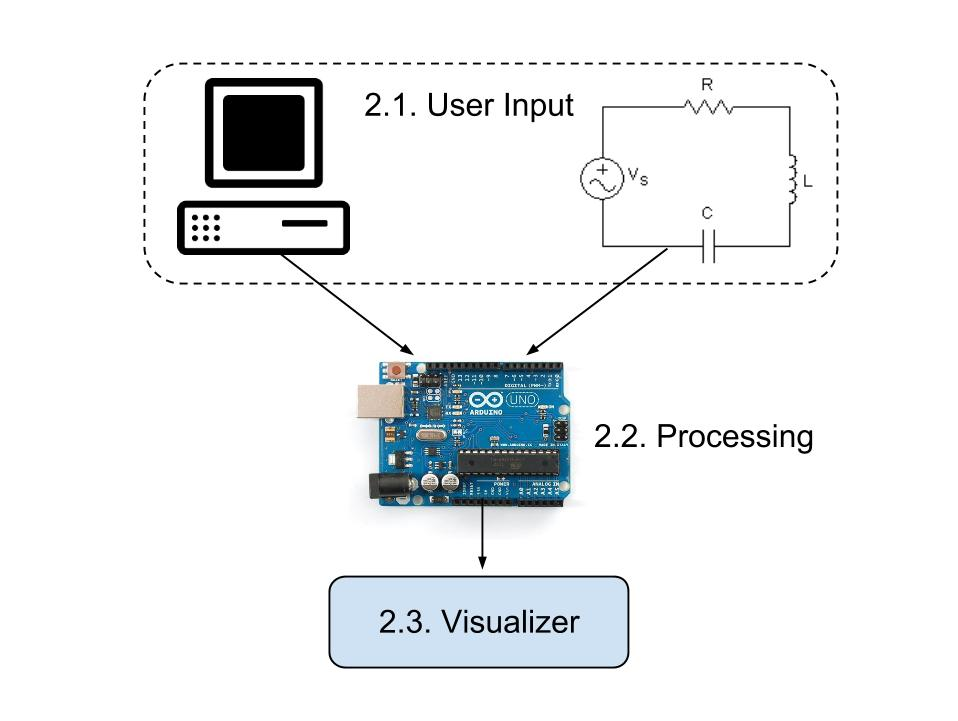
\includegraphics[height=9cm, width=12cm]{Hierarchy.jpg}
\caption{Virtual Arduino Architecture}
\label{Architecture}
\end{figure}
The following section will discuss the architectural hierarchy of the full program. The section will also partition the program into modules so it can be more easily conquered. 

\subsection{User Input}
The architecture is divided into three main parts, first part in the user input which can be in form  of text i.e Arduino code or in the form of circuitry.

\subsubsection{Computer Module}
Real-life Arduino system can be divided into two parts, Integrated development environment (IDE) and hardware. The IDE or Computer Module is where the user can write, compile and upload code onto the Arduino. This shall be implemented by using the already existing opensource Arduino IDE and redirecting its output to a virtual serial port so that this binary code can be later used for the simulation. This binary code will be transimitted down from user input to the processing module. Details about the computer mode internal workings shall be dicussed in sections 2.2 amd 2.3.

\subsubsection{Circuitry Module}
The second part of the Arduino experience is external hardware. One of the main advantages of the Arduino board is that it is easily interfaceable with most hardware components as it has built-in ADC and PWM. This module is where the user gets to experiment with hardware and connect with the Arduino board. The circuitry workspace should include an easily scalable hardware library and a circuit builder. The hardware components are divided into 3 types which are input, connectors and output. Input components are mainly sensors, connector components are wires and resistors and output components are LEDs and motors. We plan on implementing this part by using and already existing opensource simulator and upgrading its GUI and its hardware components to fit the concept of the Virtual Arduino. This will be done by adding some hardware failures scenarios and giving the simulator a more realistic GUI. The circuit output or simplification if I may say so will also be sent to the next level of the architecture for further processing and linking with Computer Module output. 

\subsection{Processing Module}
This module is the junction between the upper and lower level of the architecture. It takes the binary code from the Computer Module and translates it into actions in the Virtual Arduino processor. After evaluating the different internal components of the processor the Virtual Arduino output pins shall be assessed and this will reflect on the different output hardware components. The status of the different hardware components - whether high, low or PWM signal- shall be sent to the next level of the architecture which is the Visualizer.

\subsection{Visualizer}
This is the part where the user sees the output of his program. After the code is verified and is clear of any syntactic errors the user uploads the code onto his/her Virtual Arduino and output components start to show changes. The user will also be able to alter the environment by changing the input to the sensor and see the immediate change in the output components. 

\section{Bootloader}
\label{sec:bootloader}
\begin{figure}[h!]
\centering
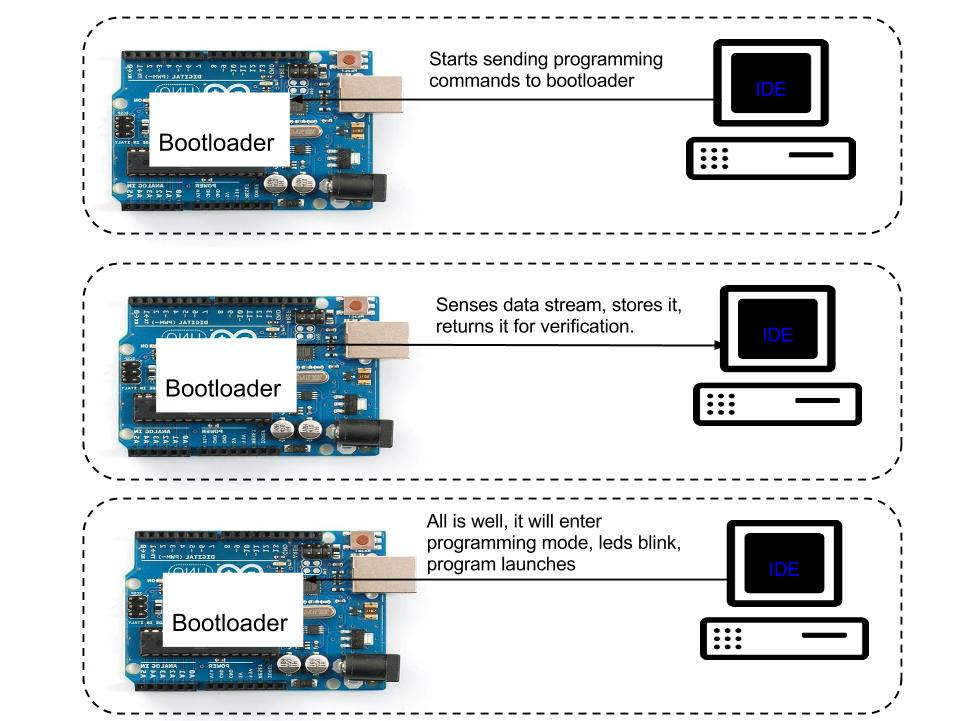
\includegraphics[height=9cm, width=12cm]{Bootloader.jpg}
\caption{Bootloader-Programmer Handshake}
\label{Bootloader Handshake}
\end{figure}
Stackoverflow \cite{Stackoverflow:URL} user \emph{angelatlarge} commented on April 3, 2013 (\href{http://stackoverflow.com/questions/15785087/upload-arduino-code-on-virtual-serial-port-through-arduino-ide/15792961?noredirect=1#comment22546153_15792961}{Upload Arduino code on virtual serial port through Arduino IDE}):
\begin{quotation}
``The process of uploading code is not a uni-directional process. There is a program on the Arduino called a bootloader [\emph{later discussed in section \ref{sec:bootloader}, the author}] which is responsible for communicating with the programmer (``programmer'': a program that programs the Arduino, assume it is the Arduino IDE for now). The Arduino CPUs cannot be programmed across serial lines. Rather these chips are programmed either via the \href{http://www.atmel.com/images/doc0943.pdf}{in system programming (ISP)} or via the \href{http://en.wikipedia.org/wiki/Jtag}{JTAG protocol}.
\end{quotation}
Retrieved from \href{http://stackoverflow.com/questions/15785087/upload-arduino-code-on-virtual-serial-port-through-arduino-ide/15792961?noredirect=1#comment22546153_15792961}{Stackoverflow}. 
Angelatlarge added  (2013, April 3).\href{http://stackoverflow.com/questions/15785087/upload-arduino-code-on-virtual-serial-port-through-arduino-ide/15792961?noredirect=1#comment22546153_15792961}{Upload Arduino code on virtual serial port through Arduino IDE} \begin{quotation}``The bootloader is a program that runs on the Arduino CPU, the program runs at startup and looks for programming commands over the serial port. If it discovers that a programmer is trying to communicate programming information, it will read the compiled Arduino binary coming over the serial link, store it in flash memory, send it back over the serial link for verification, and if everything is successful, exit and launch the stored sketch. If no programming information appears on the serial port, that is, no programmer is trying to write a new sketch, then the bootloader simply quits and launches the program already stored in flash.\end{quotation} Retrieved from http://stackoverflow.com/questions/15785087/upload-arduino-code-on-virtual-serial-port-through-arduino-ide/15792961?noredirect=1#comment22546153_15792961. 

Each Arduino board uses a different bootloader. In our program we will be simulating the ArduinoUno which uses the \href{https://github.com/arduino/Arduino/tree/master/hardware/arduino/bootloaders/optiboot}{optiboot bootloader} (publicly available on GitHub \cite{GitHub:URL}). Our plan is to mimic the responses sent from the bootloader to the IDE in order to get the code the is sent from the IDE to the flash on the Arduino board. The bootloader communicates with the IDE using the \href{http://www.atmel.com/Images/doc2525.pdf}{STK500 protocol}. The STK500 is a communication protocol of 8-bit AVR. The handshake in Figure 2.2 will also be discussed in further details in the next chapter.

\section{Communication}
In order to imitate the bootloader we had to sniff the serial port to understand what is being transmitted between the IDE and the board. First the Programmer in the IDE tries to sync with a device so it sends an GETSYNC command ([30] [20]) if a device is connected the bootloader on the device replies with INSYC, OK ([14] [10]). After establishing the connection the Programmer asks the bootloader about some of the boards specs like the hardware, firmware, system clock and reference voltage. After setting some parameters the IDE send an ENTERPROGMODE command which tells the bootloader to program the chip. The code is sent from the IDE to the board and is written in the flash memory. But before programming the chip this code has to be verified so the bootloader then sends back all what is on the flash for verification. After it is verified the chip is programmed and IDE tells the bootloader the it is done and sends an LEAVEPROGMODE command.


\section{Java Libraries}
To receive the Programmers commands and respond to them like the bootloader we had to communicate with our serial port. There are several communication libraries in Java that offer such features. Sun had a serial communication API called JavaComm but they withdrew it's support for windows in 2005. This led to the development of the free open-source \href{http://rxtx.qbang.org/wiki/index.php/Main_Page}{RxTx library}. We chose to use the Java Simple Serial Connector \href{https://code.google.com/p/java-simple-serial-connector/}{(JSSC)} library which is based on the RxTx library.

\clearpage  % Introduction ended, start a new page
